%%%

\section{Exercises}

%%%

\subsection{Small sample inference for the mean}

% The normality condition

% Introducing the t distribution

% Working with the t distribution

% The t distribution as a solution to the standard error problem

% One sample confidence intervals with small n

\eoce{An independent random sample is selected from an approximately normal population with unknown standard deviation. The sample is small ($n < 50$). Find the degrees of freedom and the critical $t$ value (t$^*$) for the given confidence level. \vspace{-3mm}
\begin{multicols}{2}
\begin{enumerate}[(a)]
\setlength{\itemsep}{0mm}
\item $n = 42$, CL = 90\%
\item $n = 21$, CL = 98\%
\item $n = 29$, CL = 95\%
\item $n = 12$, CL = 99\%
\end{enumerate}
\end{multicols}
}
{
\begin{enumerate}[(a)]
\setlength{\itemsep}{0mm}
\item $n = 42$, CL = 90\%, $df = 42 - 1 = 41$, $t^*_{41} = 1.68$
\item $n = 21$, CL = 80\%, $df = 21 - 1 = 20$, $t^*_{20} = 1.33$
\item $n = 29$, CL = 95\%, $df = 29 - 1 = 28$, $t^*_{28} = 2.05$
\item $n = 12$, CL = 99\%, $df = 12 - 1 = 11$, $t^*_{11} = 3.11$
\end{enumerate}
}

%

{\eoce{A 90\% confidence interval for a population mean is (65,77). The population distribution is approximately normal and the population standard deviation is unknown. Given that this confidence interval is calculated based on an independent random sample of size 25, calculate the sample mean, the margin of error, and the sample standard deviation.
}
{
The sample mean is the midpoint of the confidence interval: $\bar{x} = \frac{65 + 77}{2} = 71$ \\
The margin of error is half the width of the confidence interval: $ME = \frac{77 - 65}{2} = 6$ \\
Using $df = 25 - 1 = 24$ and the confidence level of 90\% we can find the critical value from the t-table: $t^*_{24} = 1.71$. Lastly, using the margin of error and the critical value we can solve for $s$:
\begin{align*}
ME &= t^*_{24} \frac{s}{\sqrt{n}} \\
6 &= 1.71 \frac{s}{\sqrt{25}} \\
&= 0.342 s \\
s &= 17.54
\end{align*}
}
}

%

\eoce{For a given confidence level, $t^*_{df}$ is larger than $z^*$. Explain how $t^{*}_{df}$ being slightly larger than $z^{*}$ affects the width of the confidence interval.}
{
With a larger critical value the confidence interval ends up being wider. This makes intuitive sense as when we have a small sample size and the population standard deviation is unknown, we should have a wider interval than if we knew the population standard deviation, or if we had a large enough sample size.
}

% One sample t tests with small n

\eoce{An independent random sample is selected from an approximately normal population with unknown standard deviation. The sample is small ($n < 50$). Find the p-value for the given set of hypotheses and $t$ values. Also determine if the null hypothesis would be rejected at $\alpha = 0.05$. \vspace{-3mm}
\begin{multicols}{2}
\begin{enumerate}[(a)]
\setlength{\itemsep}{0mm}
\item $H_A: \mu > \mu_0 $, $n = 11$, $T = 1.91$
\item $H_A: \mu < \mu_0 $, $n = 17$, $T = -3.45$
\item $H_A: \mu \ne \mu_0 $, $n = 38$, $T = 0.83$
\item $H_A: \mu > \mu_0 $, $n = 47$, $T = 2.13$
\end{enumerate}
\end{multicols}
}
{
\begin{enumerate}[(a)]
\setlength{\itemsep}{0mm}
\item $H_A: \mu > \mu_0 $, $n = 11$, $T= 1.91$, $df = 11 - 1 = 10$, $0.025 < p-value < 0.05$, Reject $H_0$
\item $H_A: \mu < \mu_0 $, $n = 17$, $T = -3.45$, $df = 17 - 1 = 16$, $p-value < 0.005$, Reject $H_0$
\item $H_A: \mu \ne \mu_0 $, $n = 38$, $T = 0.83$, $df = 38 - 1 = 37$, $p-value > 0.20$,  Fail to reject $H_0$
\item $H_A: \mu > \mu_0 $, $n = 47$, $T = 2.13$, $df = 47 - 1 = 46$, $0.01 < p-value < 0.025$, Reject $H_0$ \\
\end{enumerate}

\begin{center}
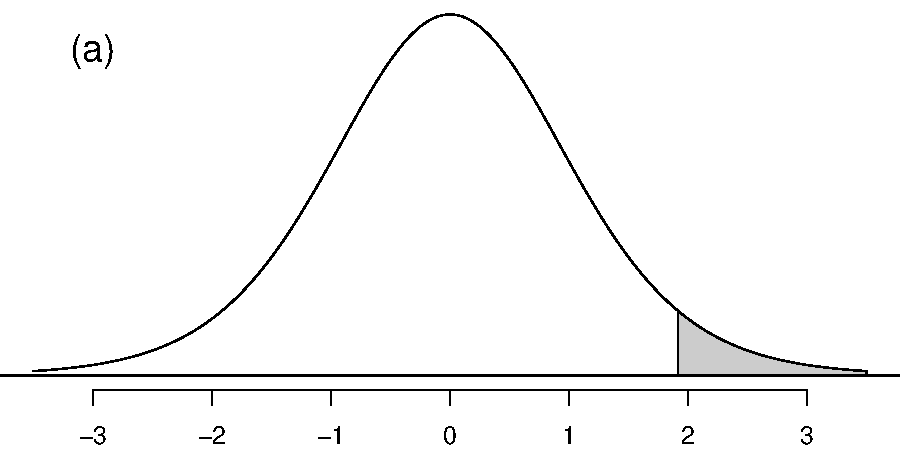
\includegraphics[width=55mm]{06/figures/eoce/oneSampleTa.pdf}
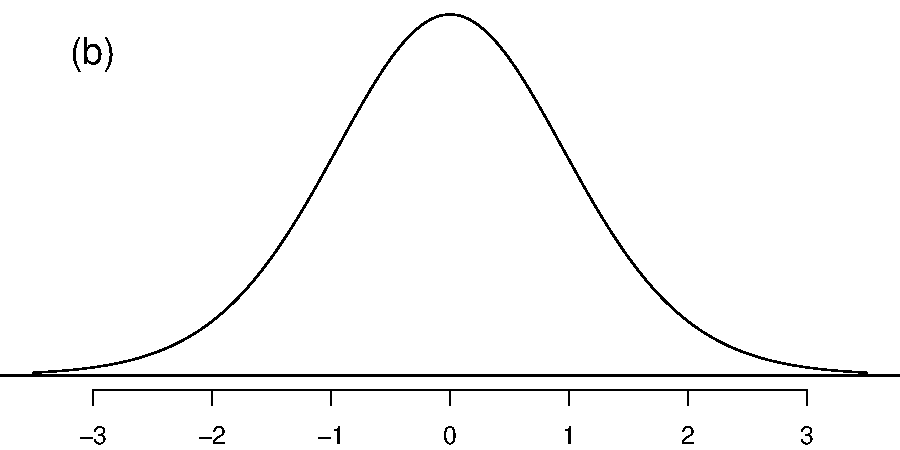
\includegraphics[width=55mm]{06/figures/eoce/oneSampleTb.pdf} \\
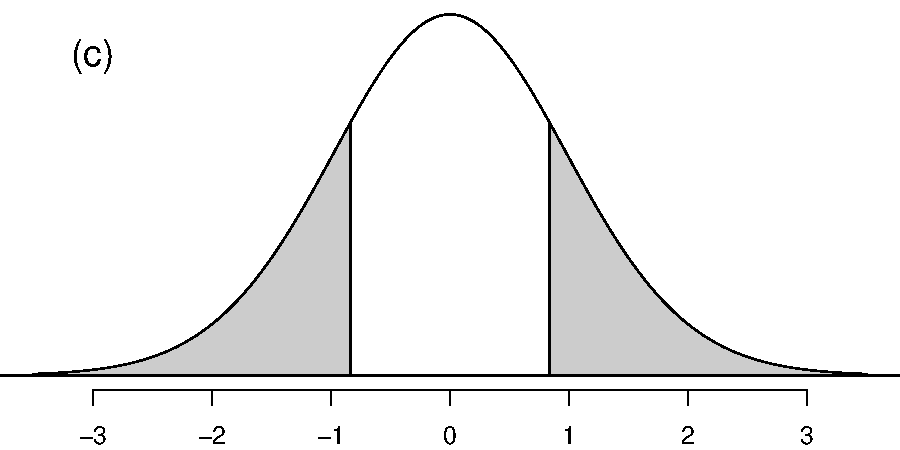
\includegraphics[width=55mm]{06/figures/eoce/oneSampleTc.pdf}
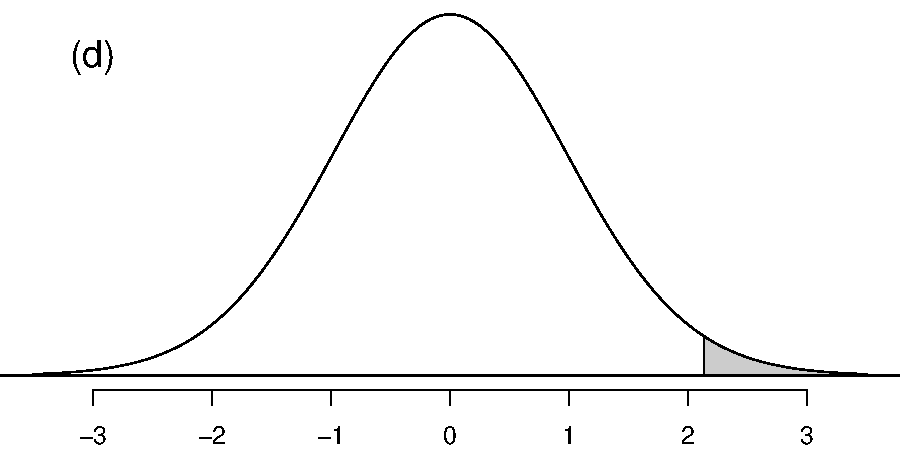
\includegraphics[width=55mm]{06/figures/eoce/oneSampleTd.pdf}
\end{center}
}

%

\eoce{
New York is known as ``the city that never sleeps". A random sample of 25 New Yorkers were asked how much sleep they get per night. A summary of some sample statistics are shown below. We are interested in finding out if these data provide convincing evidence to suggest that New Yorkers on average sleep less than 8 hours a night?
\begin{center}
\begin{tabular}{rrrrrr}
  \hline
n 	& $\bar{x}$	& s		& min 	& max \\ 
  \hline
25 	& 7.73 		& 0.77 	& 6.17 	& 9.78 \\ 
   \hline
\end{tabular}
\end{center}

\begin{enumerate}[(a)]
\setlength{\itemsep}{0mm}
\item Write the hypotheses in symbols and in words.
\item Are the assumptions/conditions for inference satisfied?
\item Calculate the test statistic, $T$.
\item Find and interpret the p-value in context. Drawing a picture may be helpful.
\item Based on the hypothesis test do these data provide convincing evidence to suggest that New Yorkers on average sleep less than 8 hours a night?
\item If we were to calculate a confidence interval at an equivalent confidence level as the hypothesis test for the true average amount of sleep Net Yorkers get per night based on this sample, would you expect it to include 8 hours? Explain. You do not actually need to calculate the confidence interval.
\end{enumerate}
}
{
\begin{enumerate}[(a)]
\setlength{\itemsep}{0mm}

\item $H_0: \mu = 8$ (New Yorkers on average sleep 8 hrs per night.) \\
$H_A: \mu < 8$ (New Yorkers on average sleep less than 8 hrs per night.)

\item 
\begin{enumerate}[1.]
\item Independence Assumption: 
\begin{itemize}
\item Random Sampling Condition: We are told that the sample is random.
\item 10\% Condition: 25 $<$ 10\% of all New Yorkers.
\end{itemize}
Since we have a random sample and the 10\% condition is satisfied, we can assume that the number of hours one New Yorker in the sample sleeps is independent of another.
\item Nearly Normal Condition: We do not have a plot of the data however we can tell that there are no extreme outliers as all observations are within 2 standard deviations of the mean.
\[ 7.73 \pm 2 * 0.77 = (6.18, 9.26) \]
If there is skew, it is not strong. There are no red flags for the normal model based on this (limited) information, and we do not have reason to believe the number of hours of New Yorkers sleep per day is not nearly normal. 
\end{enumerate}

\item The test statistic can be calculated as follows.
\begin{align*}
T &= \frac{\bar{x} - \mu_0}{\frac{s}{\sqrt{n}}} = \frac{7.73 - 8}{\frac{0.77}{\sqrt{25}}} = -1.75\\
df &= 25 - 1 = 24
\end{align*}

\item $0.025 < p-value < 0.05$

\begin{minipage}[c]{0.5\textwidth}
If in fact the true population mean of the amount New Yorkers sleep per night was 8 hours, the probability of getting a random sample of 25 New Yorkers where the average amount of sleep is 7.73 hrs per night or less is between 0.025 and 0.05.
\end{minipage}
\begin{minipage}[c]{0.5\textwidth}
\begin{center}
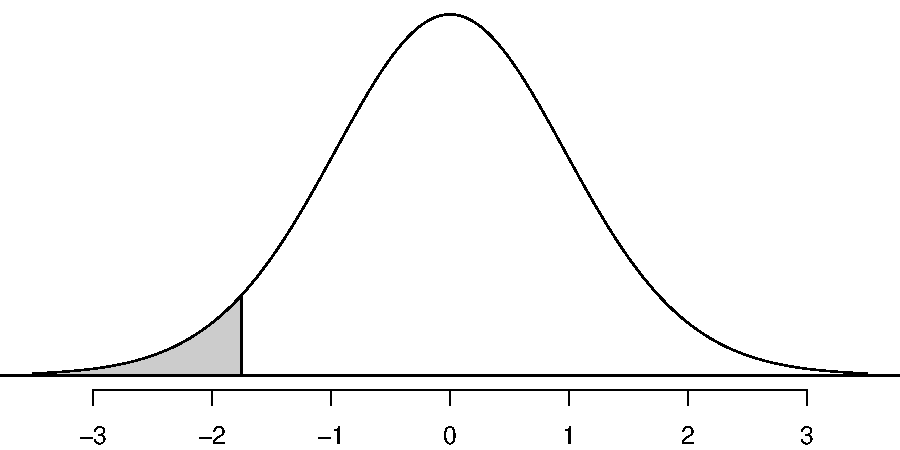
\includegraphics[width=55mm]{06/figures/eoce/newYork.pdf}
\end{center}
\end{minipage}


\item Since p-value $< \alpha$ (use $\alpha = 0.05$ since not given) we reject the null hypothesis. The data provide convincing evidence to suggest that New Yorkers on average sleep less than 8 hours per night.

\item No, the hypothesis test suggests that the average amount of sleep New Yorkers get is significantly lower than 8 hours per night, therefore we wouldn't expect 8 hours to be in the interval.

\end{enumerate}
}\label{NewYorkSleep}

%

\eoce{A recent article in a college newspaper claims that students at this college spend more than an hour per day on average on social networking sites. The article is based on a survey conducted at this college on a random sample of 45 college students which yielded a sample mean of 68.2 minutes with a standard deviation of 21 minutes. A histogram of the data is shown below. We are interested in finding out if these data provide convincing evidence to suggest that students at this college spend more than an hour (60 minutes) per day on average on social networking sites. \\
\noindent \begin{minipage}[c]{0.5\textwidth}
\begin{enumerate}[(a)]
\setlength{\itemsep}{0mm}
\item Write the hypotheses in symbols and in words.
\item Are the assumptions/conditions for inference satisfied?
\item Calculate the test statistic, $T$.
\item Find and interpret the p-value in context. Drawing a picture may be helpful.
 \newcounter{enumi_saved}
      \setcounter{enumi_saved}{\value{enumi}}
\end{enumerate}
\end{minipage}
\begin{minipage}[c]{0.5\textwidth}
\begin{center}
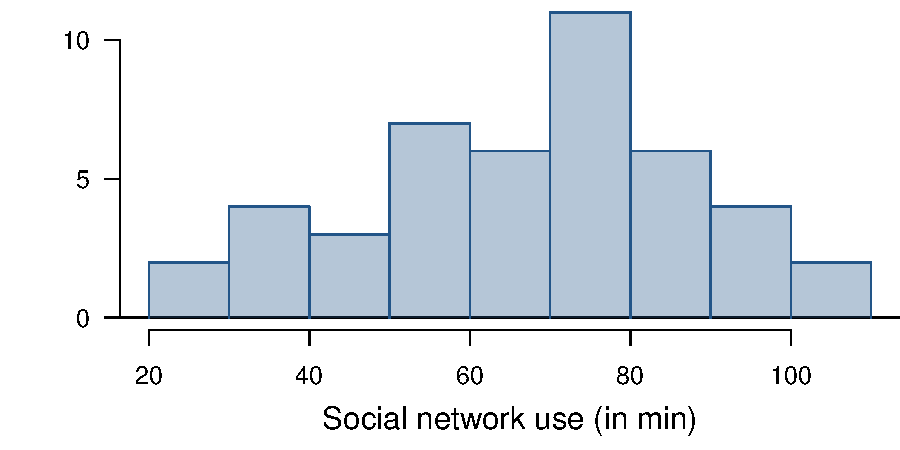
\includegraphics[width= \textwidth]{06/figures/eoce/socNetUseHist}
\end{center}
\end{minipage}
\begin{enumerate}[(a)]
\setlength{\itemsep}{0mm}
      \setcounter{enumi}{\value{enumi_saved}}
\item Based on the hypothesis test do these data provide convincing evidence to suggest students at this college spend more than an hour (60 minutes) per day on average on social networking sites.
\item If we were to calculate a confidence interval at an equivalent confidence level as the hypothesis test for the true average amount of time students at this college spend on social networking sites per day, would you expect it to include 60 minutes? Explain. You do not actually need to calculate the confidence interval.
\end{enumerate}
}
{
\begin{enumerate}[(a)]
\setlength{\itemsep}{0mm}
\item $H_0: \mu = 60$ (Students at this college spend an hour per day on average on social networking sites.) \\
$H_A: \mu > 60$ (Students at this college spend more than an hour per day on average on social networking sites.)
\item 
\begin{enumerate}[1.]
\item Independence Assumption: 
\begin{itemize}
\item Random Sampling Condition: We are told that the sample is random.
\item 10\% Condition: It is safe to assume that 45 $<$ 10\% of all students at this college.
\end{itemize}
Since we have a random sample and the 10\% condition is satisfied, we can assume that the amount of time one student in this sample spends on social networking sites is independent of another.
\item Nearly Normal Condition: The histogram does not show an extremely skewed distribution, therefore we can assume that the amount of time college students spend on social networking sites has an approximately normal distribution.
\end{enumerate}
\item The test statistic can be calculated as follows.
\begin{align*}
t &= \frac{\bar{x} - \mu_0}{\frac{s}{\sqrt{n}}} = \frac{68.2 - 60}{\frac{20}{\sqrt{45}}} = 2.75\\
df &= 45 - 1 = 44
\end{align*}
\item $p-value < 0.005$ \\
\begin{minipage}[c]{0.5\textwidth}
If in fact students at this college spend on average an hour per day on social networking sites, the probability of getting a random sample of 45 students where the average amount of time spend on social networking sites is 68.2 minutes or higher is less than 0.005.
\end{minipage}
\begin{minipage}[c]{0.5\textwidth}
\begin{center}
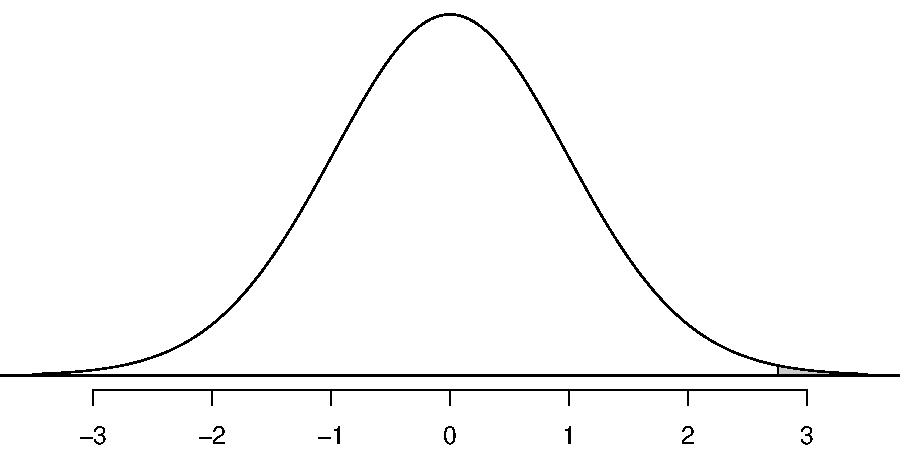
\includegraphics[width=55mm]{06/figures/eoce/socNetUse}
\end{center}
\end{minipage}
\item No, the hypothesis test suggests that the average amount of time students at this college spend on social networking sites per day is significantly higher than 60 minutes, therefore we wouldn't expect 60 minutes to be in the interval.
\end{enumerate}
}\label{socNetUse}

%

\eoce{Exercise~\eoceref{NewYorkSleep} gives some summary statistics on the number of hours of sleep 25 randomly sampled New Yorkers get per night. 
\begin{enumerate}[(a)]
\setlength{\itemsep}{0mm}
\item Calculate a 90\% confidence interval for the number of hours of New Yorkers sleep on average and interpret this interval in context.
\item Does your confidence interval agree with the result of the hypothesis test from Exercise~\eoceref{NewYorkSleep}?
\end{enumerate}
}
{
\begin{enumerate}[(a)]
\setlength{\itemsep}{0mm}
\item Before we can calculate the confidence interval, we need to find the degrees of freedom and $t^*_{df}$.
\[ df = 25 - 1 = 24 \hspace{5mm} t^*_{df} = 1.71\]

A 90\% confidence interval can be calculated as follows:
\begin{align*}
\bar{x} \pm t^*_{df} \frac{s}{\sqrt{n}} &= 7.73 \pm 1.71\frac{0.77}{\sqrt{25}} \\
&= 7.73 \pm 0.26 \\
&= (7.47, 7.99)
\end{align*}
We are 90\% confident that New Yorkers on average sleep 7.46 to 7.99 hours per night.

\item Yes, we rejected the null hypothesis and the null hypothesized value is not in the interval. It should be noted however that the upper bound of the interval is very close to 8. 

\end{enumerate}

}

%

{\eoce{Exercise~\eoceref{socNetUse} gives the mean and standard deviation of the amount of time 45 randomly sampled students at a college spend on social networking sites per day.
\begin{enumerate}[(a)]
\setlength{\itemsep}{0mm}
\item Calculate a 90\% confidence interval for the true average amount of time students at this college spend on social networking sites per day
\item Does your confidence interval agree with the result of the hypothesis test from Exercise~\eoceref{socNetUse}?
\end{enumerate}
}
{
\begin{enumerate}[(a)]
\setlength{\itemsep}{0mm}
\item Before we can calculate the confidence interval, we need to find the degrees of freedom and $t^*_{df}$.
\[ df = 45 - 1 = 44 \hspace{5mm} t^*_{df} = 1.68\]
A 90\% confidence interval can be calculated as follows:
\begin{align*}
\bar{x} \pm t^*_{df} \frac{s}{\sqrt{n}} &= 68.2 \pm 1.68\frac{21}{\sqrt{45}} \\
&= 68.2 \pm 5.25 \\
&= (62.95, 73.45)
\end{align*}
We are 90\% confident that student at this college spend on average 62.95 to 73.45 minutes per day on social networking sites.
\item Yes, we rejected the null hypothesis and the null hypothesized value is not in the interval.
\end{enumerate}
}}

%

\subsection{The t distribution for the difference of two means}

\eoce{We are interested in comparing the average total personal income in Cleveland, OH and Sacramento, CA based on a random sample of individuals from the 2000 Census. Below are a histogram representing the distributions of total personal income of individuals living in Cleveland and Sacramento and some summary statistics on the two samples. Is a t-test appropriate for testing whether or not there is a difference in the average incomes in these two metropolitan cities based on this data set? Explain. \\
\begin{minipage}[c]{0.67\textwidth}
\begin{center}
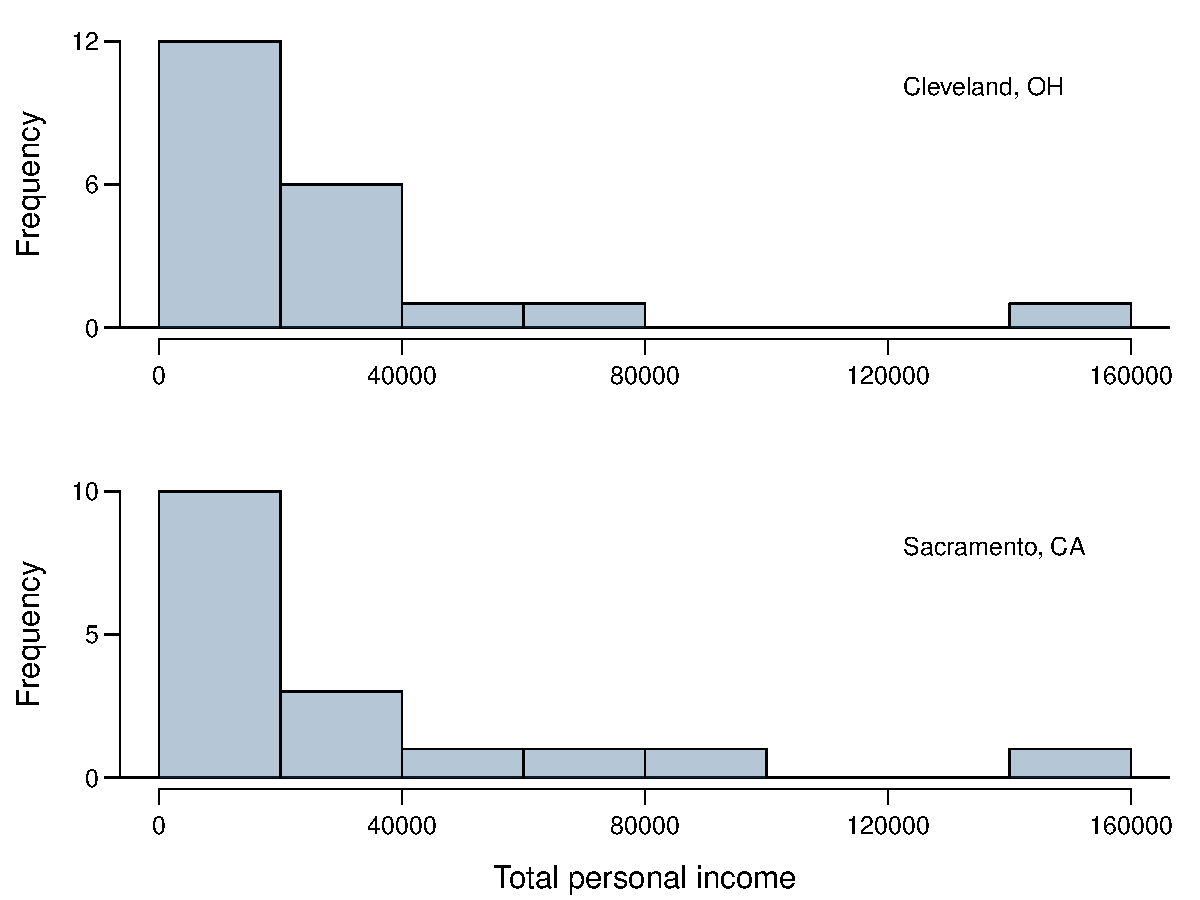
\includegraphics[width= \textwidth]{06/figures/eoce/incomeCleSac}
\end{center}
\end{minipage}
\begin{minipage}[c]{0.325\textwidth}
{\small
\begin{tabular}{l c}
\hline
		& Cleveland, OH	\\
\hline
Mean 	& \$ 26,436		\\
SD 		& \$ 33,239		\\
n 		& 21				
\end{tabular}

\vspace{2cm}

\begin{tabular}{l c}
\hline
		& Sacramento, CA \\
\hline
Mean	& \$ 32,182 \\
SD		& \$ 40,480 \\
n		& 17
\end{tabular}
}
\end{minipage}
}
{
No, a t-test is not appropriate since the distributions of total personal income are extremely skewed.
}

%

{\eoce{The first oscar award for best actor and best actress was given out in 1929. The histograms below show the age distribution for all the best actor and best actress winners from 1929 to 2011. Summary statistics for these distributions are also provided. Is a t-test appropriate for testing whether or not there is a difference in the average ages of actors and actresses who have won an Oscar in the past? Explain. \\
\begin{minipage}[c]{0.72\textwidth}
\begin{center}
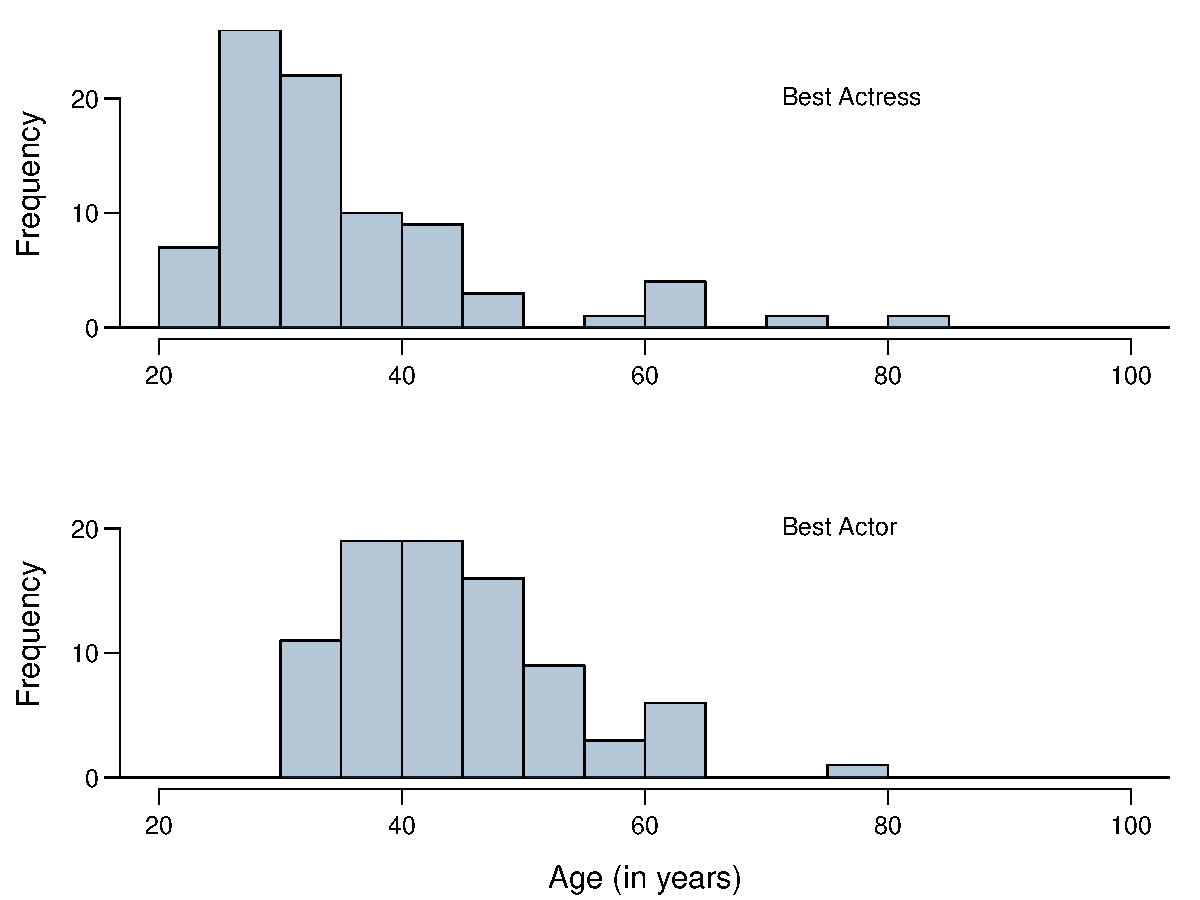
\includegraphics[width= \textwidth]{06/figures/eoce/oscarWinnersHist}
\end{center}
\end{minipage}
\begin{minipage}[c]{0.275\textwidth}
{\small
\begin{tabular}{l c}
\hline
		& Best Actress	\\
\hline
Mean 	& 35.6		\\
SD 		& 11.3		\\
n 		& 84				
\end{tabular}
$\:$ \\
\vspace{2cm}
$\:$ \\
\begin{tabular}{l c}
\hline
		& Best Actor \\
\hline
Mean	& 44.7 \\
SD		& 8.9 \\
n		& 84
\end{tabular}
}
\end{minipage}
}
{
These data come from a population (all oscar winners) not a random sample, so there is no need for hypothesis testing in this situation. We can see that the average age for the population of best actress winners is lower than the average age for the best actor winners.
}}


% A distribution for the difference of two sample means

% Two sample t test

\eoce{Two independent random samples are selected from normal populations with unknown standard deviations. Both samples are small ($n < 50$). Find the p-value for the given set of hypotheses and $t$ values. Also determine if the null hypothesis would be rejected at $\alpha = 0.05$.
\begin{enumerate}[(a)]
\setlength{\itemsep}{0mm}
\item $H_A: \mu_1 > \mu_2$, $n_1 = 23$, $n_2 = 25$, $T = 3.16$
\item $H_A: \mu_1 \ne \mu_2$, $n_1 = 38$,  $n_2 = 37$, $T = 2.72$
\item $H_A: \mu_1 < \mu_2$, $n_1 = 45$,  $n_2 = 41$, $T = 1.83$
\item $H_A: \mu_1 \ne \mu_2$, $n_1 = 11$,  $n_2 = 15$, $T = 0.28$
\end{enumerate}
}
{
\begin{enumerate}[(a)]
\setlength{\itemsep}{0mm}
\item $H_A: \mu_1 > \mu_2$, $n_1 = 23$, $n_2 = 25$, $T = 3.16$, $df = min(23 - 1, 25 - 1) = min(22, 24) = 24$, $p-value < 0.005$, Reject $H_0$.
\item $H_A: \mu_1 \ne \mu_2$, $n_1 = 38$,  $n_2 = 37$, $T = 2.70$, $df = min(38 - 1, 37 - 1) = min(37, 36) = 36$, $0.01 < p-value < 0.02$, Reject $H_0$.
\item $H_A: \mu_1 < \mu_2$, $n_1 = 45$,  $n_2 = 41$, $T = 1.83$, $df = min(45 - 1, 41 - 1) = min(44, 40) = 40$, $0.05 < p-value < 0.10$, Fail to reject $H_0$.
\item $H_A: \mu_1 \ne \mu_2$, $n_1 = 11$,  $n_2 = 15$, $T = 0.28$, $df = min(11 - 1, 15 - 1) = min(10, 14) = 10$, $p-value < 0.20$, Fail to reject $H_0$.
\end{enumerate}
}

% Two sample t confidence interval

\eoce{Two independent random samples are selected from normal populations with unknown standard deviations. Both samples are small ($n < 50$). Find the degrees of freedom and the critical $t$ value (t$^*$) for the given confidence level. Remember that a reasonable choice of degrees of freedom for the two-sample case is the minimum of $n_1-1$ and $n_2-1$. The ``exact" df is something we cannot compute from the given info. \vspace{-2.5mm}
\begin{multicols}{2}
\begin{enumerate}[(a)]
\setlength{\itemsep}{0mm}
\item $n_1 = 16$, $n_2 = 16$, CL = 90\%
\item $n_1 = 36$, $n_2 = 41$, CL = 95\%
\item $n_1 = 8$, $n_2 = 10$, CL = 99\%
\item $n_1 = 23$, $n_2 = 27$, CL = 98\%
\end{enumerate}
\end{multicols}
}
{
\begin{enumerate}[(a)]
\setlength{\itemsep}{0mm}
\item $n_1 = 16$, $n_2 = 16$, CL = 90\%, $df = min(16 - 1, 16 - 1) = min(15, 15) = 15$, $t^*_{15} =  1.75$
\item $n_1 = 36$, $n_2 = 41$, CL = 95\%, $df = min(36 - 1, 41 - 1) = min(35, 40) = 35$, $t^*_{35} =  2.03$
\item $n_1 = 10$, $n_2 = 8$, CL = 99\%, $df = min(10 - 1, 8 - 1) = min(9, 7) = 7$, $t^*_{7} =  3.50$
\item $n_1 = 23$, $n_2 = 27$, CL = 98\%, $df = min(23 - 1, 27 - 1) = min(22, 26) = 7$, $t^*_{22} =  2.51$
\end{enumerate}
}

%

\eoce{A weight loss pill claims to accelerate weight loss when accompanied with exercise and diet. Diet researchers from a consumer advocacy group decided to test this claim using an experiment. 42 subjects were randomly assigned to two groups: 21 took the pill and 21 only received a placebo. Both groups underwent the same diet and exercise regiment. In the group that got the pill the average weight loss was 20\textit{lbs} with a standard deviation of 4\textit{lbs}. In the placebo group the average weight loss was 18\textit{lbs} with a standard deviation of 5\textit{lbs}. 
\begin{enumerate}[(a)]
\setlength{\itemsep}{0mm}
\item Calculate a 95\% confidence interval for the difference between the two means.
\item Interpret the confidence interval in context.
\item Based on your confidence interval, is there significant evidence to suggest that the weight loss pill is effective?
\item Does this prove that the weight loss pill is/is not effective?
\end{enumerate}
}
{
\begin{enumerate}[(a)]
\setlength{\itemsep}{0mm}
\item Before we can calculate the confidence interval, we need to find the degrees of freedom and $t^*_{df}$.
\begin{align*}
df &= min(n_1 - 1,  n_2 - 1) = min(20,20) = 20 \\
t^*_{20} &= 2.086
\end{align*}
\begin{align*}
(\bar{x}_1 - \bar{x}_2) \pm t^*_{df}  \sqrt{\frac{s_1^2}{n_1} + \frac{s_2^2}{n_2}} &= (20 - 18) \pm 2.086 * \sqrt{\frac{4^2}{21} + \frac{5^2}{21}} \\
&= 2 \pm 2.91 \\
&= (-0.91, 4.91)
\end{align*}

\item We are 95\% confident that those in the group that got the weight loss pill lost 0.91\textit{lbs} less to 4.91\textit{lbs} more than those in the placebo group.

\item Since the confidence interval includes 0 there is no significant evidence to suggest that the weight loss pill is effective.

\item No, we can only say that the data \textit{suggest} that the pill is not effective, we did not prove that it is not. There may be other contributing factors. 
\end{enumerate}
}

%

\eoce{A company has two factories in which they manufacture engines. Once a month they randomly select 10 engines from each factory to test if there is a difference in performance in engines made in the two factories. The average output of the motors from Factory 1 is 120 horsepower with a standard deviation of 5 horsepower.  The average output of the motors from Factory 2 is 132 horsepower with a standard deviation of 4 horsepower.  
\begin{enumerate}[(a)]
\setlength{\itemsep}{0mm}
\item Calculate a 95\% confidence interval for the difference in the average horsepower for engines coming from the two factories.
\item Interpret the confidence interval in context.
\item Based on your confidence interval, is there significant evidence to suggest that there is a difference in performance in engines made in the two factories? If so, can you tell which factory produces motors with lower performance? Explain.
\item Recently upgrades were made in Factory 2.  Does this prove that these upgrades enhanced the performance in engines made in the this factory? Explain.
\end{enumerate}
}
{
\begin{enumerate}[(a)]
\setlength{\itemsep}{0mm}

\item Before we can calculate the confidence interval, we need to find the degrees of freedom and $t^*_{df}$.
\begin{align*}
df &= min(n_1 - 1,  n_2 - 1) = min(9,9) = 9 \\
t^*_{9} &= 2.262
\end{align*}
\begin{align*}
(\bar{x}_1 - \bar{x}_2) \pm t^*_{df}  \sqrt{\frac{s_1^2}{n_1} + \frac{s_2^2}{n_2}} &= (120 - 132) \pm 2.262 * \sqrt{\frac{5^2}{10} + \frac{4^2}{10}} \\
&= -12 \pm 4.58 \\
&= (-16.58, -7.42)
\end{align*}

\item We are 95\% confident that average output of the motors made in Factory 1 is 7.42 to 16.58 horsepower lower than the motors made in Factory 2.

\item Yes, since the confidence interval does not include 0 there is significant evidence to suggest that there is a difference in performance in engines made in the two factories. Factory 1 produces motors with lower performance.

\item Even though there seems to be a statistically significant difference in the performances of engines made in the two factories, we can't tell if the upgrades made in Factory 2 \textit{caused} this. There may be other contributing factors.

\end{enumerate}
}

%

\eoce{An experiment was conducted to measure and compare the effectiveness of various feed supplements on the growth rate of chickens. Newly hatched chicks were randomly allocated into six groups, and each group was given a different feed supplement. Their weights in grams after six weeks are given along with feed types in the data set called \texttt{chickwts} \citep{data:chickwts}. Below are some summary statistics from this data set along with box plots  showing the distribution of weights by feed type. \\
\noindent\begin{minipage}[c]{0.635\textwidth}
\begin{center}
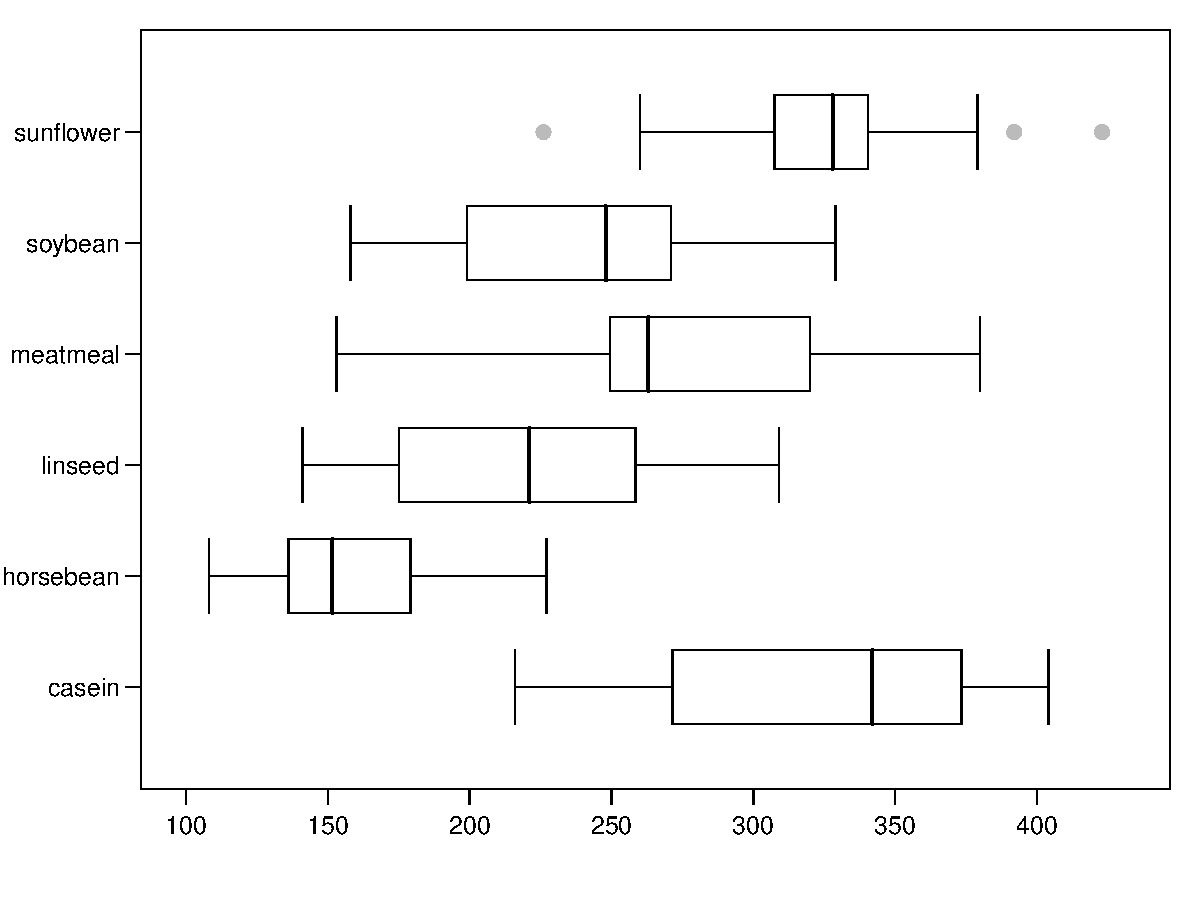
\includegraphics[width= \textwidth]{06/figures/eoce/chickwts.pdf}
\end{center}
\end{minipage}
\begin{minipage}[c]{0.36\textwidth}
{\footnotesize\begin{tabular}{l c c c}
\hline
              		& Mean		& SD		& n \\
\hline
casein    		& 323.58 		& 64.43	& 12 \\
horsebean 	& 160.20 		& 38.63	& 10 \\
linseed   		& 218.75 		& 52.24	& 12 \\
meatmeal  	& 276.91 		& 64.90	& 11 \\
soybean   		& 246.43 		& 54.13	& 14 \\
sunflower 		& 328.92 		& 48.84	& 12 \\
\hline
\end{tabular}}
\end{minipage} \vspace{-6mm}
\begin{enumerate}[(a)]
\setlength{\itemsep}{0mm}

\item Describe the distributions of weights of chicken that were fed linseed and horsebean.

\item Write the hypotheses for testing for a significant difference between the average weights of chicken that were fed linseed and horsebean.

\item Are the assumptions and conditions for inference satisfied?

\item Calculate the test statistic and find the p-value.

\item Using $\alpha = 0.05$ what do you conclude? Interpret your conclusion in context.

\item What type of error might we have committed? Explain.

\item Would your conclusion change if we used $\alpha = 0.01$?

\end{enumerate}
}
{
\begin{enumerate}[(a)]
\setlength{\itemsep}{0mm}

\item Chicken that were fed linseed on average weigh 218.75 grams while those that were given horsebean weigh on average 160.20 grams. Both distributions are relatively symmetric with no apparent outliers. Weights of chicken that were fed horsebean range from about 100 grams to 225 grams, and weights of chicken that were fed horsebean range from about 150 grams to 300 grams. There is a lot more variability in the weights of chicken that were given linseed.

\item Let linseed be group 1 and horsebean be group 2. Then,\\
$H_0: \mu_1 = \mu_2$ \\
$H_0: \mu_1 \ne \mu_2$ \\

\item Assumptions and conditions:
\begin{enumerate}[1.]
\item Independence Assumption: 
\begin{itemize}
\item Random Sampling Condition: We are told that chickens are randomly assigned to feed groups.
\item 10\% Condition: 12 and 10 $<$ 10\% of all chickens fed linseed and horsebean.
\end{itemize}
Since we have random samples and the 10\% condition is satisfied for both samples, we can assume that the weights of chicken fed linseed  are independent of each other, as well as the weights of chicken fed horsebean.
\item Nearly Normal Condition: We can see from the box plots that the distributions of weights of chicken in the two samples are pretty symmetric.
\item Independent Groups: Since assignment is done randomly the two samples are independent of each other.
\end{enumerate}

\item Since population standard deviations are unknown and samples are small we calculate a t score.

\[ T = \frac{(\bar{x}_1 - \bar{x_2}) - (\mu_1 - \mu_2)}{\sqrt{ \frac{s_1^2}{n_1} + \frac{s_2}{n_2} }} = \frac{(218.75 - 160.20) - 0}{ \sqrt{\frac{52.24^2}{12} + \frac{38.63^2}{10}} } = 3.02 \]
\[ df = min(n_1 - 1,  n_2 - 1) = min(11,10) = 10 \]
\[ p-value = P(|t| > 3.02) \rightarrow 0.01 < p-value < 0.02  \]

\item Since p-value $< \alpha$, reject $H_0$. The data provide convincing evidence to suggest that there is a significant difference between the average weights of chicken that were fed linseed and horsebean.

\item Type I, since we rejected $H_0$.

\item Yes, since p-value$> 0.01$, we would fail to reject $H_0$ and conclude that there isn't a significant difference between the average weights of chicken that were fed linseed and horsebean.

\end{enumerate}
}\label{chickwts}

%

\eoce{Casein is a common weight gain supplement for humans. Does it have the same effect on chicken? Using data provided in Exercise~\eoceref{chickwts} test the hypothesis that the average weight of chickens that were fed casein is higher than the average weight of chickens that were fed soybean. Assume that conditions for inference are satisfied and the data are symmetrically distributed.
}
{
Let casein be group 1 and soybean be group 2. Then,
$H_0: \mu_1 = \mu_2$ \\
$H_0: \mu_1 > \mu_2$ \\
\[ t = \frac{(\bar{x}_1 - \bar{x_2}) - (\mu_1 - \mu_2)}{\sqrt{ \frac{s_1^2}{n_1} + \frac{s_2}{n_2} }} = \frac{(323.58 - 246.43) - 0}{ \sqrt{\frac{64.43^2}{12} + \frac{54.13^2}{10}} } = 3.05 \]
\[ df = min(n_1 - 1,  n_2 - 1) = min(11,13) = 11 \]
\[ p-value = P(t > 3.05) \rightarrow 0.005 < p-value < 0.01  \]
Since p-value $< \alpha$ (use $\alpha = 0.05$ since not given), reject $H_0$. There is sufficient evidence to suggest that there average weight of chickens that were fed casein is higher than the average weight of chickens that were fed soybean.
}

%

\eoce{Each year the US Environmental Protection Agency (EPA) releases fuel economy data on cars manufactured in that year \citep{data:epaMPG2010}. Below are some summary statistics on fuel efficiency (in miles/gallon) random samples of cars with manual and automatic transmission cars manufactured in 2010. Based on this information, is there a significant difference between the average fuel efficiency of cars with manual and automatic transmission in terms of their city mileage? Assume that conditions for inference are satisfied and the data are symmetrically distributed. \vspace{-1.5mm}
\begin{center}
{\footnotesize\begin{tabular}{l c c c c c}
\hline
              		& Mean City MPG 	& SD City MPG 	& Mean Hwy MPG	& SD Hwy MPG  	& n \\
\hline
Manual    		& 21.08        		& 4.29        		& 29.31       		& 4.63 			& 26 \\
Automatic 	& 15.62        		& 2.76        		& 21.38       		& 3.73 			& 26 \\
\hline
\end{tabular}}
\end{center}
}
{
Let manual be group 1 and automatic be group 2. Then,
$H_0: \mu_1 = \mu_2$ \\
$H_0: \mu_1 \ne \mu_2$ \\
Since population standard deviations are unknown and samples are small we calculate a T score.

\[ t = \frac{(\bar{x}_1 - \bar{x_2}) - (\mu_1 - \mu_2)}{\sqrt{ \frac{s_1^2}{n_1} + \frac{s_2}{n_2} }} = \frac{(21.08 - 15.62) - 0}{ \sqrt{\frac{4.29^2}{26} + \frac{2.76^2}{26}} } = 5.46 \]
\[ df = min(n_1 - 1,  n_2 - 1) = min(26 - 1, 26 - 1) = 25 \]
\[ p-value = P(|t| > 5.6) < 0.01  \]
Since p-value $< \alpha$ (use $\alpha = 0.05$ since not given), reject $H_0$. The data provide convincing evidence to suggest that there a significant difference between the average fuel efficiency of cars with manual and automatic transmission in terms of their city mileage.
}\label{epaMPG2010}

%

\eoce{An organization studying the gender gap in starting pay for people with bachelor's degrees randomly samples 28 women and 24 men who recently graduated from Big Ten Universities.  The average starting pay for the women surveyed is \$38,293.78 per year with a standard deviation of \$5,170.22 while average starting pay for the men surveyed is \$41,981.82 per year with a standard deviation of \$3,195.42. Do these data provide convincing evidence that there is a difference between the average starting salaries for men and women with bachelor's degrees? Assume that conditions for inference are satisfied and the data are symmetrically distributed and use $\alpha= 0.02$. \\
}
{
Let women be group 1 and men be group 2. Then, \\
$H_0: \mu_{1} = \mu_{2}$, The average starting salaries for women and men are equal. \\
$H_A: \mu_{1} \ne \mu_{2}$, The average starting salaries for women and men are different. \\
Since population standard deviations are unknown and samples are small we calculate a T score.
\[ t = \frac{(\bar{x}_1 - \bar{x_2}) - (\mu_1 - \mu_2)}{\sqrt{ \frac{s_1^2}{n_1} + \frac{s_2}{n_2} }} = \frac{(38,293.78 - 41,981.82) - 0}{ \sqrt{\frac{5,170.22 ^2}{28} + \frac{3,195.42 ^2}{24}} } = -3.14 \]
\[ df = min(n_1 - 1,  n_2 - 1) = min(28 - 1, 24 - 1) = 23 \]
\[ p-value < 0.01 \]
Since p-value $<$ 0.02, we reject $H_0$. The data provide convincing evidence of a difference between the average starting salaries for men and women who who recently graduated from Big Ten Universities with bachelor's degrees.}\label{menWomenSalaries}

%

{\eoce{Exercise~\eoceref{epaMPG2010} provides data on fuel efficiency of cars manufactured in 2010. Use these statistics to calculate a 95\% confidence interval for the difference between average highway mileage of manual and automatic cars and interpret this interval in context.
}
{
\begin{align*}
df &= min(n_1 - 1,  n_2 - 1) = min(26 - 1, 26 - 1) = 25 \\
t^*_{25} &= 2.06
\end{align*}
\begin{align*}
(\bar{x}_1 - \bar{x}_2) \pm t^*_{df}  \sqrt{\frac{s_1^2}{n_1} + \frac{s_2^2}{n_2}} &= (29.31 - 21.37) \pm 2.06 * \sqrt{\frac{4.63^2}{26} + \frac{3.73^2}{26}} \\
&= 7.93 \pm 2.80 \\
&= (5.13, 10.73)
\end{align*}
We are 95\% confident that cars with manual transmission on average get 5.13 to 10.73 miles per gallon more than cars with automatic transmission.
}}

%

\eoce{Exercise~\eoceref{menWomenSalaries} provides some summary statistics on the starting salaries of men and women who recently graduated from Big Ten Universities. Based on this information, calculate a 98\% confidence interval for the difference between the average starting salaries of such men and women and interpret this interval in context.
}
{
\begin{align*}
df &= min(n_1 - 1,  n_2 - 1) = min(28 - 1, 24 - 1) = 23 \\
t^*_{23} &= 2.50
\end{align*}
\begin{align*}
(\bar{x}_1 - \bar{x}_2) \pm t^*_{df}  \sqrt{\frac{s_1^2}{n_1} + \frac{s_2^2}{n_2}} &= (38,293.78 - 41,981.82) \pm 2.50 * \sqrt{\frac{5,170.22 ^2}{28} + \frac{3,195.42 ^2}{24}} \\
&= -3,688.04 \pm 1,174.79 \\
&= (2,513.25, 4,862.83)
\end{align*}
We are 98\% confident that men who recently graduated from Big Ten Universities with bachelor's degrees make \$2,513.25 to \$4,862.83 per year more than women with an equivalent educational background.
}

%

\subsection{Small sample hypothesis testing for a proportion}

{\eoce{A popular uprising that started on January 25, 2011 in Egypt led to the 2011 Egyptian Revolution. Polls show that about 69\% of American adults followed the news about the political crisis and demonstrations in Egypt closely during the first couple weeks following the start of the uprise \citep{web:egypt}. Among a random sample of 30 high school students, it was found that only 17 of them followed the news about Egypt closely during this time. 
\begin{enumerate}[(a)]
\setlength{\itemsep}{0mm}
\item Write the hypotheses for testing if the proportion of high school students who followed the news about Egypt is lower than the proportion of American adults who did.
\item Calculate the proportion of high schoolers in this sample who followed the news about Egypt closely during this time.
\item For large sample theory, we modeled $\hat{p}$ using the normal distribution. Why is this not appropriate here?
\item Since using the normal distribution is not appropriate, we would like to test this hypothesis using a simulation. Describe a setup for a simulation test that would be appropriate in this situation and how the p-value can be calculated using the simulation results.
\item Below is a histogram showing the distribution of $\hat{p}_{sim}$ in 10,000 simulations under the null hypothesis. Estimate the p-value using the plot and determine the conclusion of the hypothesis test.
\begin{center}
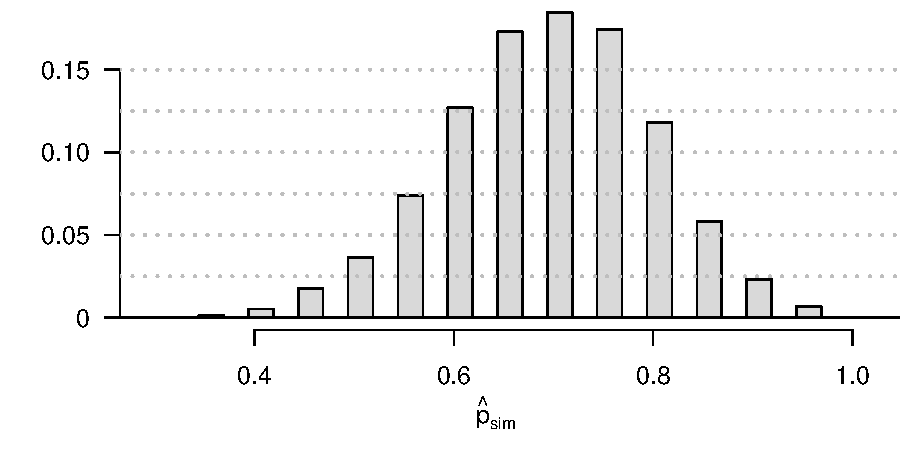
\includegraphics[width=0.8\textwidth]{06/figures/eoce/egypt}
\end{center}
\end{enumerate}
}
{
\begin{enumerate}[(a)]
\setlength{\itemsep}{0mm}
\item $H_0: p = 0.69$ \\
$H_A: p < 0.69$
\item $\hat{p} = \frac{17}{30} = 0.57$
\item The success-failure condition is not satisfied. Under the null hypothesis, we would expect to have 30*0.69 = 20.7 high school students to follow the news and 30*0.31 = 9.3 to not follow the news, not the 10 required for the normal approximation.
\item Each student can be represented with a card. Take 100 cards, 69 black cards representing those who follow the news about Egypt and 31 red cards representing those who do not. Shuffle the cards and draw 30 cards representing the 30 high school students. Calculate the proportion of black cards in this sample, $\hat{p}_{sim}$, i.e. the proportion of those who follow the news. Repeat 10,000 times and plot the resulting sample proportions. The p-value will be the proportion of simulations where $\hat{p}_{sim} \le 0.57$.
\item The p-value is represented by the area shown below in blue. In 1,348 out of the 10,000 $\hat{p}_{sim} \le 0.57$, therefore p-value $= \frac{1348}{10000} = 0.1348$. (Note that students may have approximate results.) 
\noindent \begin{minipage}[c]{0.5\textwidth}
Since p-value is high, we fail to reject $H_0$. The data do not provide convincing evidence that the proportion of high school students who followed the news about Egypt is lower than the proportion of American adults who did. 
\end{minipage}
\begin{minipage}[c]{0.5\textwidth}
\begin{center}
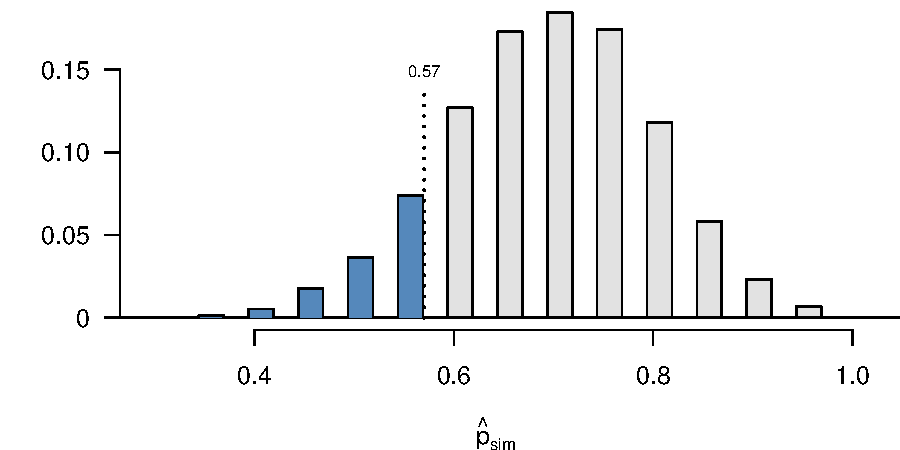
\includegraphics[width= 0.9\textwidth]{06/figures/eoce/egyptSoln}
\end{center}
\end{minipage}
\end{enumerate}
}
}

%

{\eoce{Assisted Reproductive Technology (ART) is a collection of techniques that help facilitate pregnancy (e.g. in vitro fertilization). A 2008 report by the Centers for Disease Control estimated that ART has been successful in leading to a live birth in 31\% of cases \citep{web:art}. A new infertility clinic claims that their success rate is higher than average. A random sample of 30 of their patients yielded a success rate of 40\%.
\begin{enumerate}[(a)]
\setlength{\itemsep}{0mm}
\item Write the hypotheses to test if the success rate for ART at this clinic is significantly higher than the average success rate.
\item For large sample theory, we modeled $\hat{p}$ using the normal distribution. Why is this not appropriate here?
\item Since using the normal distribution we would like to test this hypothesis using a simulation. Describe a setup for a simulation test that would be appropriate in this situation and how the p-value can be calculated using the simulation results.
\item Below is a histogram showing the distribution of $\hat{p}_{sim}$ in 10,000 simulations under the null hypothesis. Estimate the p-value using the plot and determine the conclusion of the hypothesis test.
\begin{center}
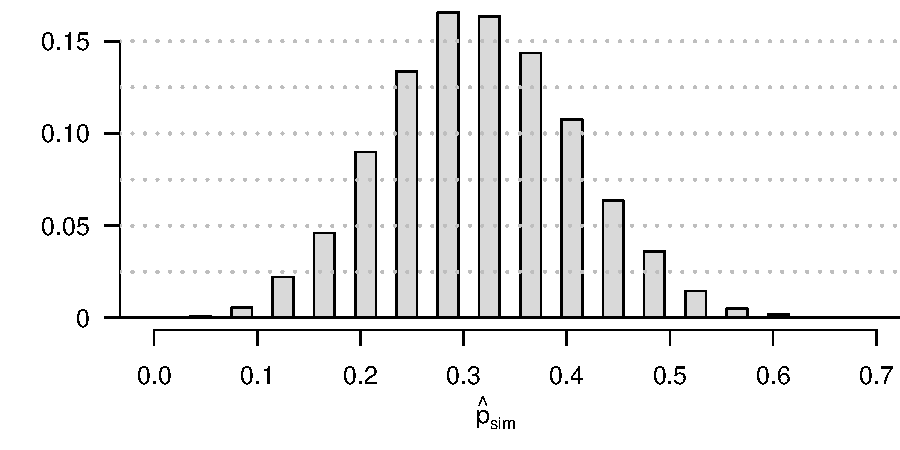
\includegraphics[width=0.8\textwidth]{06/figures/eoce/art}
\end{center}
\end{enumerate}
}
{
\begin{enumerate}[(a)]
\setlength{\itemsep}{0mm}
\item $H_0: p = 0.31$ \\
$H_A: p > 0.31$
\item The success-failure condition is not satisfied. Under the null hypothesis, we would expect to have 25*0.31 = 7.75 
live births, not the 10 required for the normal approximation.
\item Each patient can be represented with a card. Take 100 cards, 31 black cards representing successful ART cycles  and 69 red cards representing unsuccessful ART cycles. Shuffle the cards and draw 25 cards representing these patients. Calculate the proportion of black cards in this sample, $\hat{p}_{sim}$, i.e. the proportion of successful ART cycles. Repeat 10,000 times and plot the resulting sample proportions. The p-value will be the proportion of simulations where $\hat{p}_{sim} \ge 0.40$.
\item The p-value is represented by the area shown below in blue. In 2,285out of the 10,000 $\hat{p}_{sim} > 0.40$, therefore p-value $= \frac{1158}{10000} = 0.2285$. (Note that students may have approximate results.) 
\noindent \begin{minipage}[c]{0.5\textwidth}
Since p-value is high, we fail to reject $H_0$. The data do not provide convincing evidence that the the success rate for ART at this clinic is significantly higher than the average success rate.
\end{minipage}
\begin{minipage}[c]{0.5\textwidth}
\begin{center}
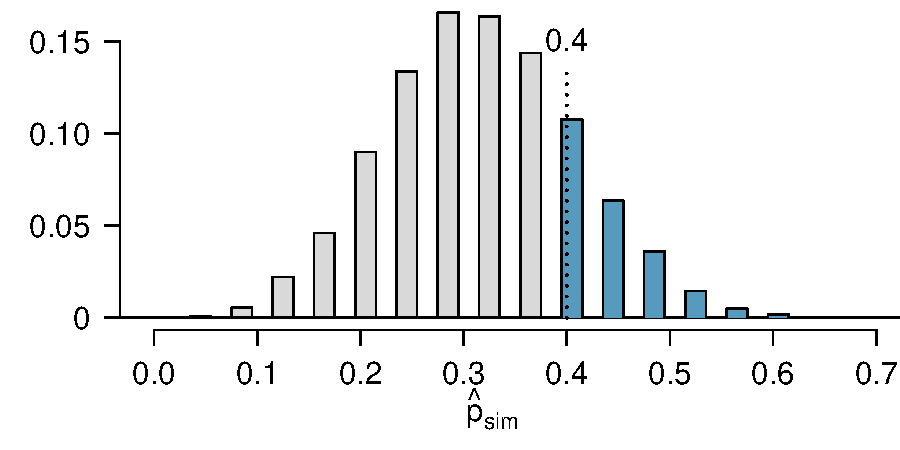
\includegraphics[width= 0.9\textwidth]{06/figures/eoce/artSoln}
\end{center}
\end{minipage}
\end{enumerate}
}
}

%

\subsection{Hypothesis testing for two proportions}

{
\eoce{A ``social experiment" conducted by a TV program questioned what people do when they see a very obviously bruised woman getting picked on by her boyfriend. On two different occasions at the same restaurant the same couple was depicted, however in one scenario the woman was dressed ``provocatively" and in the other scenario the woman was dressed ``conservatively". The table below shows how many restaurant diners were present under each scenario, and whether or not they intervened.
\begin{center}
\begin{tabular}{ll  cc c} 
			&				& \multicolumn{2}{c}{\textit{Scenario}} \\
\cline{3-4}
							&			& Provocative	& Conservative 	& Total	\\
\cline{2-5}
\multirow{2}{*}{\textit{Intervene}}	&Yes 		& 5	 	& 15		& 20 	\\
							&No			& 15	 	& 10 	 	& 25 \\
\cline{2-5}
							&Total		& 20		& 25		& 45 \\
\end{tabular}
\end{center}
A randomization test was used to determine if people react differently under the two scenarios. In order to conduct the test a researcher wrote yes on 20 index cards and no on 25 index cards to indicate whether or not a diner (represented by each card) intervened. Then he shuffled the cards and dealt them into two groups of size 20 and 25, the provocative and conservative scenarios, respectively. He counted how many diners in each scenario intervened, calculated the difference between the simulated proportions of intervention as $\hat{p}_{pr,sim} - \hat{p}_{con,sim}$. This simulation was repeated 10,000 times using software to obtain 10,000 differences that are due to chance alone. The histogram below shows the distribution of the simulated differences.
\begin{center}
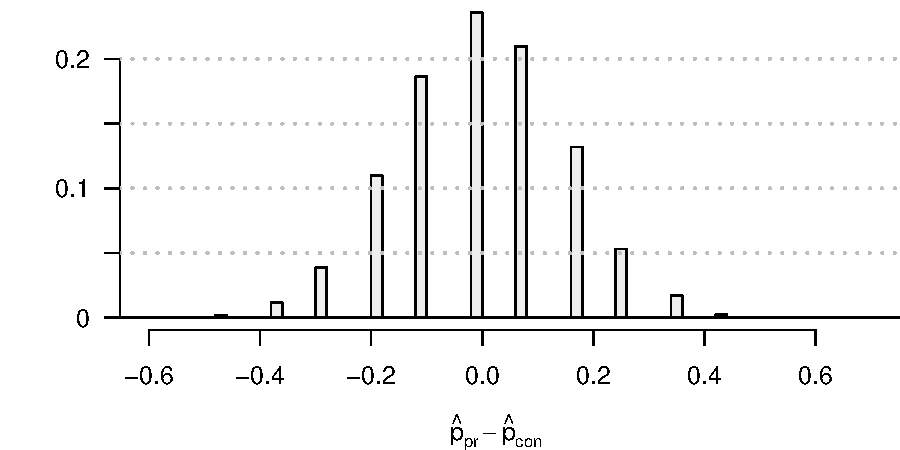
\includegraphics[width=0.8\textwidth]{06/figures/eoce/socExp}
\end{center}
\begin{enumerate}[(a)]
\setlength{\itemsep}{0mm}
\item What are the hypotheses?
\item Calculate the observed difference between the rates of intervention under the two scenarios.
\item Estimate the p-value using the figure above and determine the conclusion of the hypothesis test.
\end{enumerate}
}
{
\begin{enumerate}[(a)]
\setlength{\itemsep}{0mm}
\item $H_0: p_{provocative} = p_{conservative}$ \\
$H_A: p_{provocative} \ne p_{conservative}$
\item $\frac{5}{20} - \frac{15}{25} = -0.35$
\item The p-value is represented by the area shown below in blue. In 143 out of the 10,000 simulations differences under the null hypothesis was less than or equal to 0.35. Since the hypothesis test is two sided, p-value = $2 * \frac{143}{10000}$ = 0.0286.(Note that students may have approximate results.)
\noindent \begin{minipage}[c]{0.5\textwidth}
Since p-value is low, we reject $H_0$. The data provide convincing evidence that people react differently under the two scenarios.
\end{minipage}
\begin{minipage}[c]{0.5\textwidth}
\begin{center}
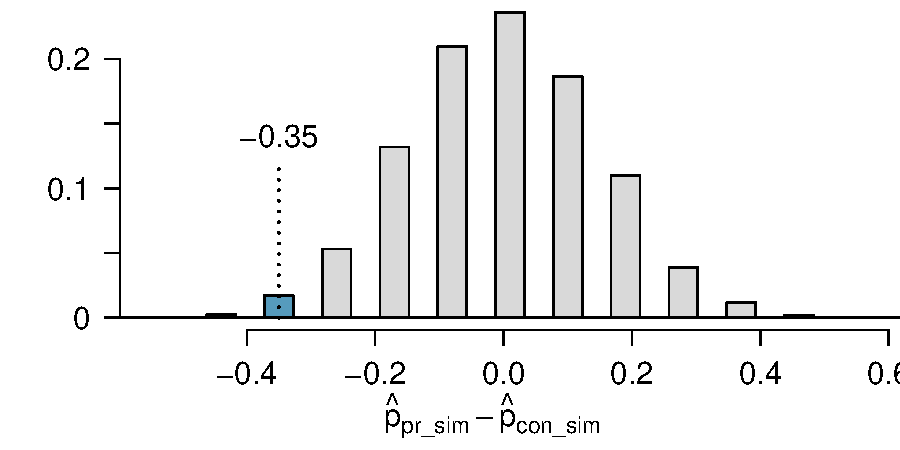
\includegraphics[width= 0.9\textwidth]{06/figures/eoce/socExpSoln}
\end{center}
\end{minipage}
\end{enumerate}
}
}

%



%%%%

%\bibliographystyle{ieeetr}
%\bibliography{chp6ex}	
